\documentclass{beamer}
\usepackage{subfig}
\usepackage{amsmath}
\usepackage{bm}

\DeclareMathOperator*{\argmax}{arg\,max}
\DeclareMathOperator*{\argmin}{arg\,min}


\title{Genetic Algorithms}
\author{Prof. Alessandro Lucantonio}
\institute{Aarhus University - Department of Mechanical and Production Engineering}
\date{?/?/2023}

\begin{document}
	\frame{\titlepage}
	
	\begin{frame}
		\frametitle{An example - The one-max problem}
		Consider the problem of maximizing the number of digits of a bitstring of length $N$. This problem is called \textbf{one-max problem}.
		
		\vspace{5mm}
		
		Formally, we can describe this problem as follows. Find a string $x = [x_1, \dots, x_N]$ with $x_i \in \{0,1\}$ that maximizes 
		\begin{equation*}
			F(x) := \sum_{i=1}^{N} x_i
		\end{equation*}
	
		Clearly, the optimal solution is the string with all bits equal to $1$, but this is the most famous benchmark of \textbf{genetic algorithms} (GA).
	\end{frame}

	\begin{frame}
		\begin{figure}
			\centering
			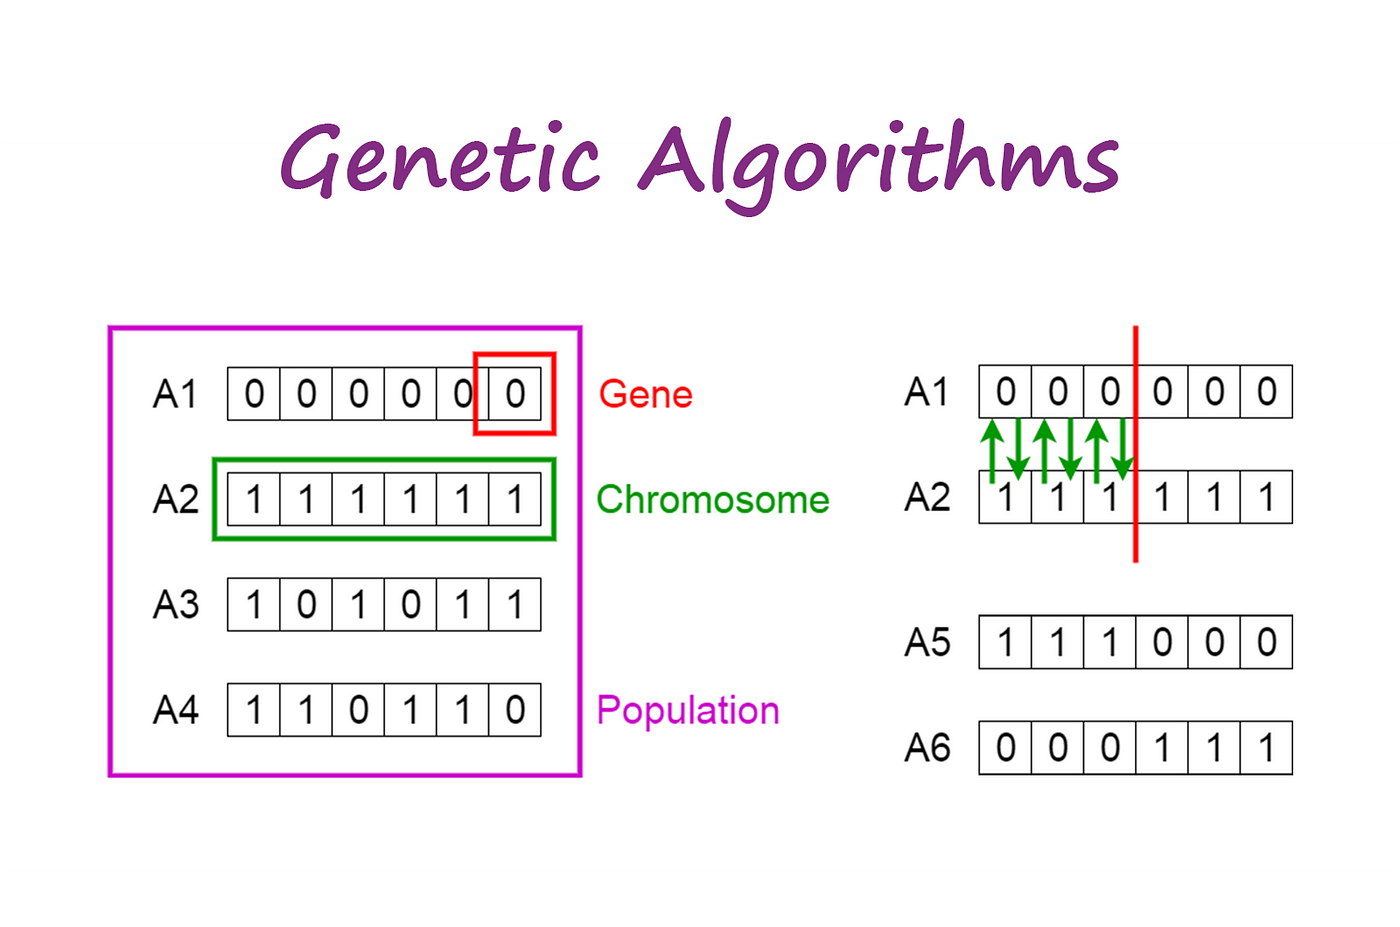
\includegraphics[scale=0.23]{images/ga}
		\end{figure}
	\end{frame}

	\begin{frame}
		\frametitle{GA - Some properties}
		\begin{itemize}
			\setlength\itemsep{5mm}
			\item Highly inspired by biological evolution.
			\item Gradient-free optimization solver.
			\item Good choice when the problem is constantly changing.
			\item Good choice when the search space is too large.
			\item Simply to develop
		\end{itemize}
	\end{frame}

	\begin{frame}
		\frametitle{Basic terminology}
		\begin{itemize}
			\item \textbf{Population}. A collection of candidate solutions.
			\item \textbf{Individual}. A possible solution to a given problem. It is also called \textbf{chromosome}.
			\item \textbf{Gene}. The indivisible building block making up an individual.
			\item \textbf{Mutation}. The operation in which genes in an individual are randomly altered to create new traits.
			\item \textbf{Crossover}. The operation in which different individuals are combined to create a new candidate solution.
			\item \textbf{Selection}. The operation that picks individuals to breed the next generation.
			\item \textbf{Fitness}. The objective function to be maximized. It is a score that measure how good is an individual.
		\end{itemize}
	\end{frame}

	\begin{frame}
		\frametitle{GA general scheme}
		\begin{figure}
			\centering
			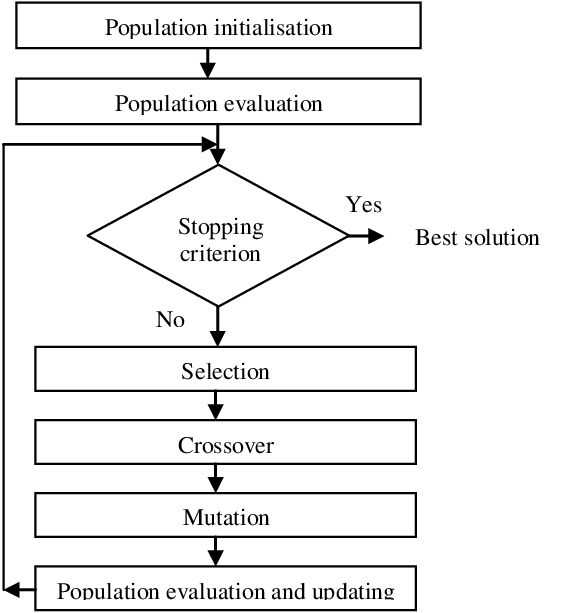
\includegraphics[scale=0.3]{images/ga_scheme}
		\end{figure}
		
	\end{frame}
	
	\begin{frame}
		\frametitle{GA general scheme}
		GA starts with an initial population, i.e. a set of individuals. Usually the population is generate randomly, to provide a uniform coverage of the search space.
		
		\begin{figure}
			\centering
			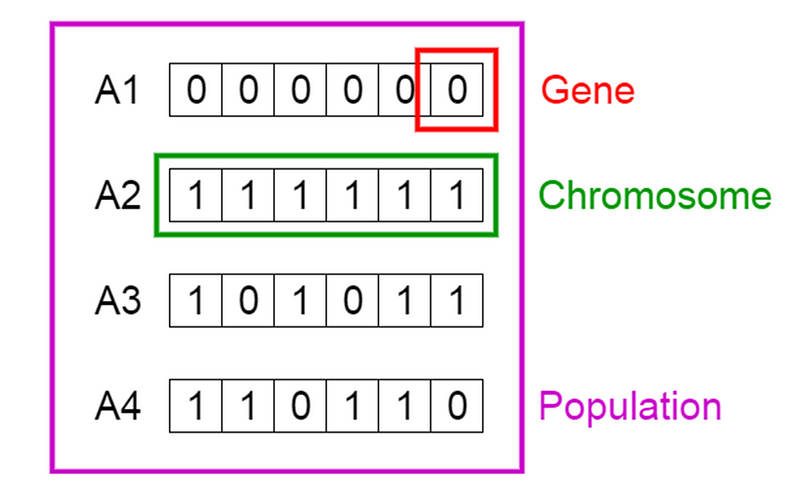
\includegraphics[scale=0.3]{images/ga_pop}
		\end{figure}
		Next, we compute the fitness function on each individual.
	\end{frame}

	\begin{frame}
		\frametitle{GA general scheme}
		After this stage, the algorithm decides whether we should terminate or not, based on a termination criteria. This is an optional step: we can choose to stop the evolution after a fixed number of generations.
		
		\vspace{5mm}
		
		Next, the individuals are selected according to a selection operation. The higher the fitness of an individual, the higher is the probability to select it.
		
		\vspace{5mm}
		
		Then, apply crossover and mutation operations to the selected individuals to create new ones. Finally, the new population goes back to evaluation phase and the process starts again.
	\end{frame}

	\begin{frame}
		\frametitle{A variant}
		In the general scheme, the new population completely replace the old one, even though the best fitness decrease.
		
		\vspace{5mm}
		
		A variation of the GA scheme that takes in account this fact works as follows. Let $n$ be the starting population size. After the evaluation process we generate $n$ new individuals by crossover and mutation. Finally, we select the $n$ best individuals among the $2n$ (old population + new individuals generated).
		
		\vspace{5mm}
		
		In this way the best fitness of each generation consists of the best fitness found so far. 
	\end{frame}
\end{document}